\chapter{相关研究概述}
无线传感网在环境监测、工业控制、资源监测和军事侦察等领域都有重要的应用,具有非常良好的前景。但是区别于传统的网络,无线传感器节点一般都部署在无人值守的环境恶劣地区或敌对区域,可能受到敌人的攻击破坏,所以安全问题十分突出。同时由于无线传感器节点的存储空间和计算能力的限制,安全机制的复杂性受到约束,因此设计适合无线传感网应用需求的安全机制十分重要。

本章首先对无线传感网的安全技术进行概述,然后对无线传感网的认证机制及其密钥分配方案进行概述。

\section{无线传感网安全技术概述}
无线传感网的节点一般部署在无人值守区域,使得无线传感网的安全问题尤为突出,特别是在军事侦察等应用领域。无线传感网不能直接沿用传统无线网络的安全机制,设计无线传感网的安全机制时,必须考虑到无线传感器网的如下限制
\upcite{c1:limitation}:
\begin{compactitem}
  \item 节点的存储空间、计算能力和通信能力有限,特别是节点的能量有限,严重制约了安全机制的发展。
  \item 无线传感网有无线自组网的缺点,缺乏基础设施建设,节点之间使用不安全的无线通信。
  \item 部署的位置一般是敌对区域或者危险区域,节点很容易受到物理攻击或者破坏。
\end{compactitem}

无线传感网的应用决定了其安全目标与传统网络有所不同,更侧重于保护感知的数据,保证数据的安全。
在无线传感网中,安全技术的目标主要包括\upcite{c1:attack}:
\begin{compactitem}
  \item 数据认证:通过认证确保数据来自经过身份认证的节点,保证数据的安全。
  \item 数据保密:确保只有通过认证的节点才能获取消息中的内容,不会暴露保密的内容。
  \item 数据完整性:确保所有受到的消息没有被未经授权的设备所篡改。
  \item 可用性:确保传感器节点在受到攻击时仍然能提供指定的基本服务。
  \item 数据新鲜:保证数据在指定时间内到达目的节点,确保数据的有效性。
\end{compactitem}

\subsection{无线传感网面临的安全威胁}

无线传感网的协议栈包括传输层、网络层、链路层和物理层,各层都会遭到不同的攻击。对于各层的攻击,有各种防御手段来保护无线传感网的安全,传输层主要研究认证机制及面向认证的密钥管理技术,网络层主要研究路由安全协议,数据链路层主要研究数据帧的安全传输,物理层主要研究节点间通信信道安全。
无线传感网中常见的攻击与防御措施\upcite{c1:attack}如表~\ref{tb:wsnattack}所示:

\begin{table}[htbp]
  \centering
  \caption{无线传感网常见的攻击与防御措施}
  \label{tb:wsnattack}
  \begin{minipage}[t]{0.8\textwidth}
    \begin{tabularx}{\linewidth}{|c|c|X|}
      \hline
%      \multirow{1}*{网络层次}
%        & 常见的攻击 & 防范措施\\
      \multirow{1}*{网络层次}  & \multicolumn{1}{c|}{常见的攻击} & \multicolumn{1}{c|}{防范措施}\\
      \hline
      \multirow{2}*{传输层}
        & 泛洪攻击 & 用户询问 \\\cline{2-3}
        & 同步破坏攻击 & 认证机制 \\
      \hline
      \multirow{7}*{网络层}
        & 泛洪攻击 & 广播和组播半径限制 \\\cline{2-3}
        & 黑洞攻击 & 节点身份认证,冗余路径 \\\cline{2-3}
        & 错误定向攻击 & 数据帧转发签名 \\\cline{2-3}
        & 蠕虫洞攻击 & 基于信任等级的路由 \\\cline{2-3}
        & 创建路由环 & 篡改校验、认证 \\\cline{2-3}
        & 汇聚节点攻击 & 加密、逐跳认证机制 \\\cline{2-3}
        & 虚假路由攻击 & 冗余机制、数据一致性检测 \\
      \hline
      \multirow{3}*{数据链路层}
        & 资源耗尽攻击 & 限制通信速度,竞争门限控制 \\\cline{2-3}
        & 碰撞攻击 & 纠错校验码 \\\cline{2-3}
        & 非公平竞争攻击 & 使用非优先级策略 \\
      \hline
      \multirow{3}*{物理层}
        & 拥塞攻击 & 使用优先级消息、宽频通信、间歇通信 \\\cline{2-3}
        & 无线干扰 & 变频通信、跳频通信 \\\cline{2-3}
        & 物理破坏 & 节点伪装和隐藏 \\
      \hline
    \end{tabularx}\\[2pt]
  \end{minipage}
\end{table}

物理层受到的攻击主要包括拥塞攻击、无线干扰和物理破坏。拥塞攻击是物理层最常见的攻击,Xu 等就提出了4种不同的拥塞攻击方法\upcite{c1:jamming},能够使无线传感网停止工作。无线干扰是干扰传感器节点的通信信道,和拥塞攻击一样都能严重影响节点的数据发送和接收。通过物理攻击,篡改节点信息是物理层的另一种攻击方法,攻击者能获得节点的内存信息,包括密钥和加密数据,从而破坏该节点的工作。

数据链路层容易受到碰撞攻击,攻击者利用协议的漏洞,在无线传感网发送大量的干扰数据包,与正常数据包传输发生碰撞,造成无线传感网正常数据无法传输,并且消耗节点能量。数据链路层还容易受到资源耗尽攻击,即向特定节点发送大量数据,消耗其节点能量,使之失效。非公平竞争是指攻击者通过发送高优先级的数据包,在网络中一直占据通信信道,使得正常节点一直无法使用信道,无法发送数据。

在无线传感网中,大量的传感器节点部署在监测区域内,报文需要经过多跳才能到达基站,无线传感网的特性决定了它没有固定的拓扑结构,所以每个节点都能进行路由,因此攻击者可以利用该特点发动网络层攻击。网络层受到的攻击包括泛洪攻击、黑洞攻击、错误定向攻击、蠕虫洞攻击、创建路由环攻击、汇聚节点攻击和虚假路由攻击。

传输层受到的攻击包括泛洪攻击和同步破坏攻击。当攻击者发送大量的连接请求,就能严重影响到无线传感网的通信,甚至无法进行正常网络通信,也就是泛洪攻击。同步破坏攻击是指向建立了通信连接的节点不断发送伪造的发送失败消息,使节点一直因为帧丢失而进行重传,而且达到攻击传感器网络的目的。

无线传感网各个协议栈都容易受到攻击,虽然都有相应的防御的措施,但是现阶段的安全机制方案还不够完善,严重制约了无线传感网的应用和发展。


\subsection{无线传感网现有的安全技术}

无线传感网面临着多种攻击的威胁,许多安全技术方案在保护其安全方面已经有了突破。
对于无线传感网的安全技术,在保证数据传输安全的前提下,其设计要考虑到如下需求:
\begin{compactitem}
  \item 稳定性:整个无线传感网的安全体系不会因为个别节点的失效或者被攻击而瘫痪。
  \item 可扩展性:传感网加入新节点,不会对原有的安全体系造成影响,同时不应产生过大的计算开销。
  \item 灵活性:安全技术不能影响到网络的部署结构的灵活性。
  \item 低开销:安全技术的计算开销、通信开销和存储开销应当适合无线传感器节点的能力,不会影响到节点的正常功能。
\end{compactitem}


无线传感网现有的安全技术主要包括加密算法、安全路由、数据聚合、入侵检测、认证机制和密钥管理,其中认证机制和密钥管理将在2.2节与2.3节进行详细论述。

\subsubsection{密码算法}
由于无线传感器节点自身的局限性,计算能力和节点存储空间有限,导致目前非对称密码算法在传感器节点不能直接应用。而对称密码算法需要的计算能力更小,存储空间开销也相对较小,因而目前的传感器网络主要使用的是对称密码算法。如RC5\upcite{c1:RC5}、RC6\upcite{c1:RC6}、Camellia\upcite{c1:Camellia}、TEA\upcite{c1:TEA} 和MISTY1\upcite{c1:MISTY1}等对称加密应用在无线传感网中,在文献\cite{c1:encryptionCompare}中,Law等对这些对称加密算法在无线传感器节点中的运行性能进行了比较和分析。

虽然现阶段非对称密码还很少应用在无线传感网的安全协议中,但是随着硬件技术的进步,传感器节点的计算和存储能力不断提高,低开销的非对称密码算法应用在无线传感网的安全协议中成为了可能,也成为了现阶段无线传感网密码算法研究的热点。现阶段非对称密码在传感器节点上的尝试主要是基于椭圆曲线的密码算法(ECC),David等将ECC应用在TinyOS中
\upcite{c1:EC},Gura等将ECC和RSA在MICA上成功实现\upcite{c1:ECC},并对它们进行了分析比较。
\subsubsection{安全路由}
路由技术在传统的网络中有非常成熟的协议,但是由于无线传感网的特性,没有特定的路由节点,每个节点都要完成路由的功能,导致无线传感网的路由技术与传统网络有较大区别。现阶段多数路由协议都注重提高路由效率,以降低节点的能量消耗,但是这样也造成了潜在的安全问题。

许多相关研究都针对无线传感网的路由安全问题进行了探索,如Deepak等提出的多路由机制\upcite{c1:multiroute},通过在多条路径上传输同一个数据报文,来防御选择性转发攻击,但是该方案中,数据报文需要传输多次,造成通信开销的浪费。还有其他路由协议通过加密和认证等方法提高路由的安全性能,如Karlof等人的方案\upcite{c1:Karlof03}和Li等人的方案
\upcite{c1:Li}。
\subsubsection{数据聚合}
数据聚合减少了无线传感网中的冗余数据,降低了通信开销,节约了节点能量。通过数据聚合安全机制,提高了无线传感网中数据私密性,提高了网络传输的安全性。

Priyanka等人在数据聚合中添加了错误数据检测机制,提出了一种高效的数据聚合方案\upcite{c1:Priyanka},保证了数据的安全传输。类似的研究还有Suat等人的方案\upcite{c1:suat},通过将数据聚合和安全传输以及错误报文过滤相结合,提高了无线传感网数据传输的安全。

Sivagami等人提出的方案\upcite{c1:Sivagami} 中,通过多节点对之间延迟发送消息认证码来对发送的数据进行认证,实现了安全的数据聚合,并且降低了传输开销。

Zhu等人提出了一种错误数据报文过滤机制\upcite{c1:zhu},通过节点间的交叉认证,保证了错误报文在被捕获节点不超过设计参数的情况下会在路径中被过滤。

\subsubsection{入侵检测}
当无线传感器节点的部署在敌对区域时,很容易受到攻击,节点被捕获或者受损不可避免,而攻击者可以通过这些妥协节点发送进一步的攻击,从而影响整个无线传感网的安全。因此在无线传感网中,入侵检测技术可以发现网络中的异常情况,并识别恶意节点,成为了无线传感网的重要安全技术手段。入侵检测主要通过对传感网中的数据发送行为和数据报文进行分析,发现异常事件,并确定恶意行为的来源节点。

无线传感网的入侵检测机制主要由入侵检测、入侵跟踪和入侵相应3部分构成。在Wang等人提出的方案中\upcite{c1:wang},构建了覆盖可疑节点及其相邻节点的支配树,通过同可疑节点的相邻节点进行合作,来判断可疑节点是失效节点或者是恶意节点,并通过使用基于覆盖的启发式技术来提升检测效率。

恶意节点检测方案还有Mathews等人的检测方案\upcite{c4:mathews2007detecting},Zhang等人提出的基于位置的妥协节点检测机制\upcite{c1:zhang},以及Agah等提出的基于非合作博弈的入侵检测方案\upcite{c1:Agah}。

\section{无线传感网认证机制概述}
无线传感网的核心功能是在目标区域采集数据,并将数据传输到数据中心。攻击者通常会针对部分节点进行攻击,在捕获节点以后,利用这些节点联合对整个无线传感网进行攻击,因此认证机制在保证无线传感网数据安全传输中发挥重要作用。认证机制按照不同的方法,可以分为对称密钥和非对称密钥认证机制、消息认证和身份认证机制或广播认证和单播认证机制。在本节中,主要讨论无线传感网的数据认证和身份认证。

\subsection{无线传感网数据认证概述}
无线传感网的数据认证有基于对称密钥和基于非对称密钥两种,因为节点的性能限制,基于对称密钥的数据认证在无线传感网中应用还不多,现阶段的方案主要是基于对称密钥实现。

现阶段的数据认证方案主要是Perrig等人提出的$\mu TESLA$方案\upcite{c1:Tesla},以及一系列基于$\mu TESLA$的改进方案。
\begin{figure}[htbp]
  \centering
  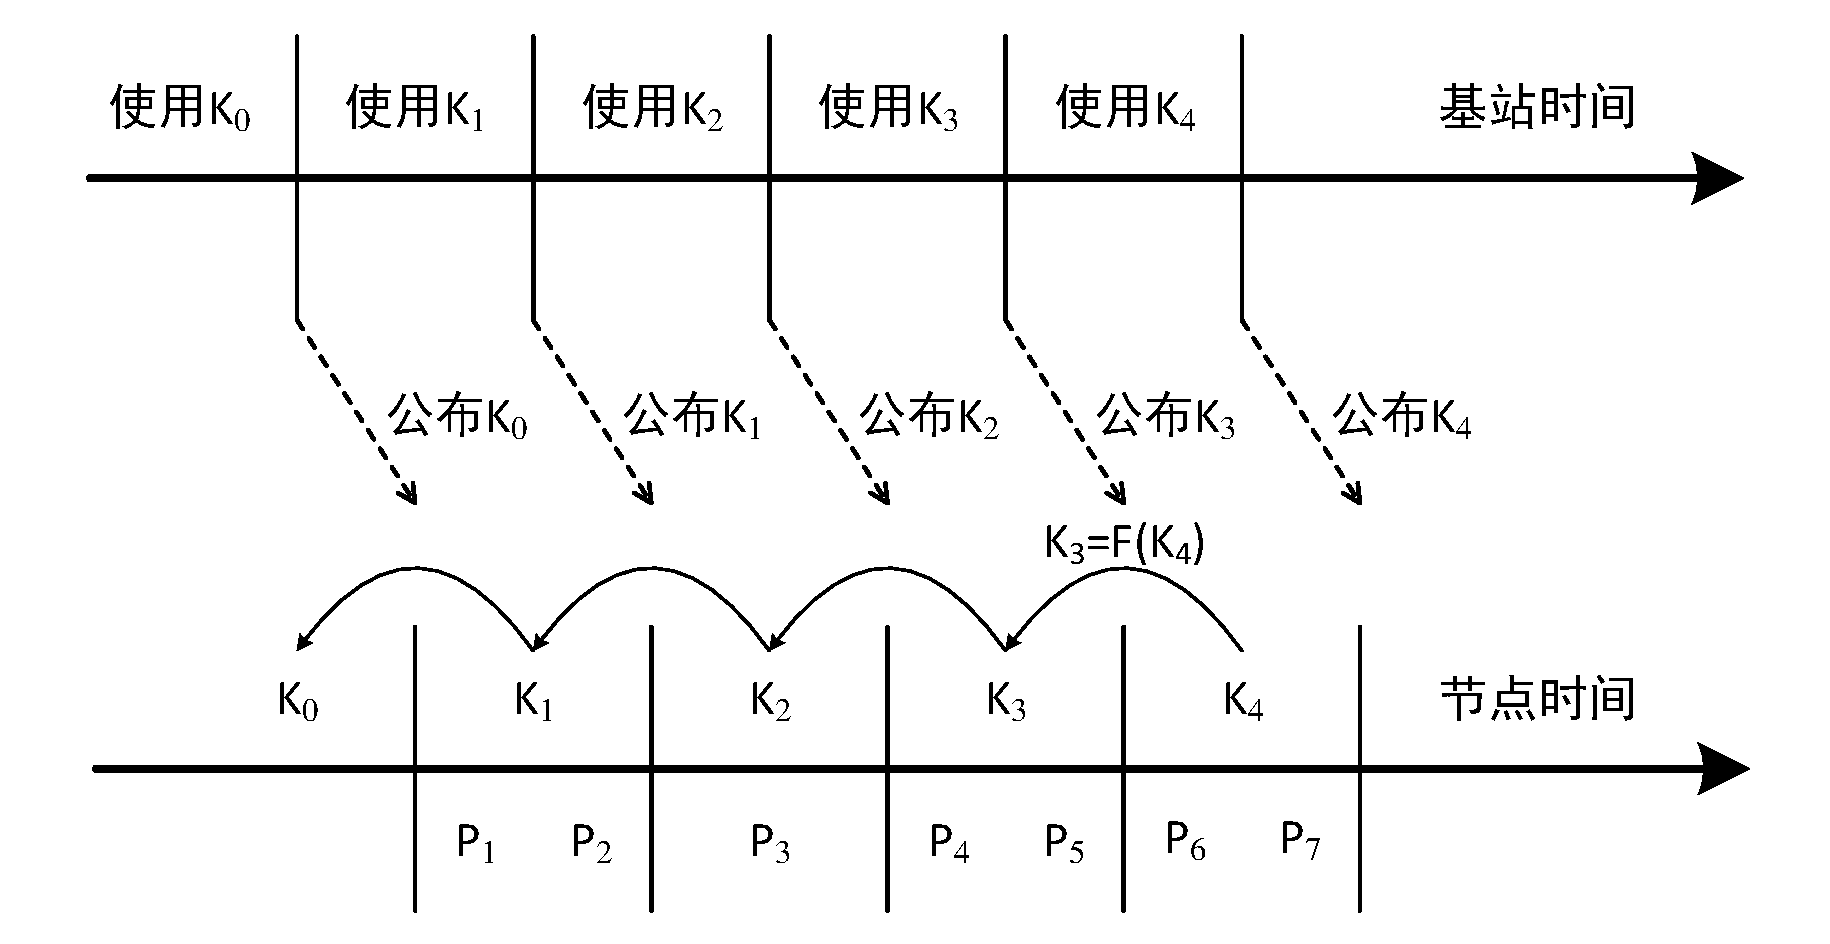
\includegraphics[width=5in]{TESLA}
  \caption{$\mu TESLA$认证机制}
  \label{fig:TESLA}
\end{figure}
如图~\ref{fig:TESLA}所示,是$\mu TESLA$方案的认证过程,$\mu TESLA$是基于对称密钥的,对报文计算消息认证码的认证密钥和节点对报文进行认证的密钥是相同的。其认证过程包括密钥建立、广播报文、自举接收者和对报文认证等步骤。其中密钥分发是通过单向hash 函数F 来实现的,如$K_3=F(K_4)$。 然后广播一个密钥$K_i$加密后的报文,无线传感网中基站和节点采用不同的时隙,使广播加密报文和接收到相应的密钥不同步。通过延迟发布密钥$K_i$,使得认证过程具有非对称性,提高认证的安全性能。通过比较报文的接收时间和认证密钥发布的时隙,能对报文的安全性进行检查。但该方案仍有其缺点:密钥的发布延后于报文的到达,因此节点接收到的报文必须缓存在节点中,浪费节点宝贵的存储空间,并且有可能被攻击者发动泛洪攻击,大量的伪造报文填满传感器节点的缓存空间,导致无线传感网传输功能失效,攻击者也容易发动虫洞攻击,威胁传感网的安全。

Liu等人基于$\mu TESLA$方案,提出了多级$\mu TESLA$方案\upcite{c1:MultiTesla},采用多级密钥链解决$\mu TESLA$方案中密钥链占用存储空间过大,容易导致泛洪攻击的问题。该方案使用预装初始化参数的方案,代替$\mu TESLA$方案中通过单播进行初始化的过程。如图~\ref{fig:MultiTESLA},是多级$\mu TESLA$方案的认证过程。在该方案中,Liu使用了2级时间,在1级时间中,将时间划分为$n_0$个间隔,每个时间间隔对应该级的单向hash链中的密钥$K_i,1\leq i \leq n_0$,其中密钥还是同$\mu TESLA$ 方案,使用单向hash链生成。一个1级时间间隔又被划分为$n_1$个2级时间间隔,每个2级时间间隔的密钥使用
$K_i,1\leq i \leq n_0$作为密钥种子生成。每个2级时间间隔内发送的报文用对应的密钥进行认证,其中的密钥链头$K_i,0$ 在前一个1级时间发布。
\begin{figure}[htbp]
  \centering
  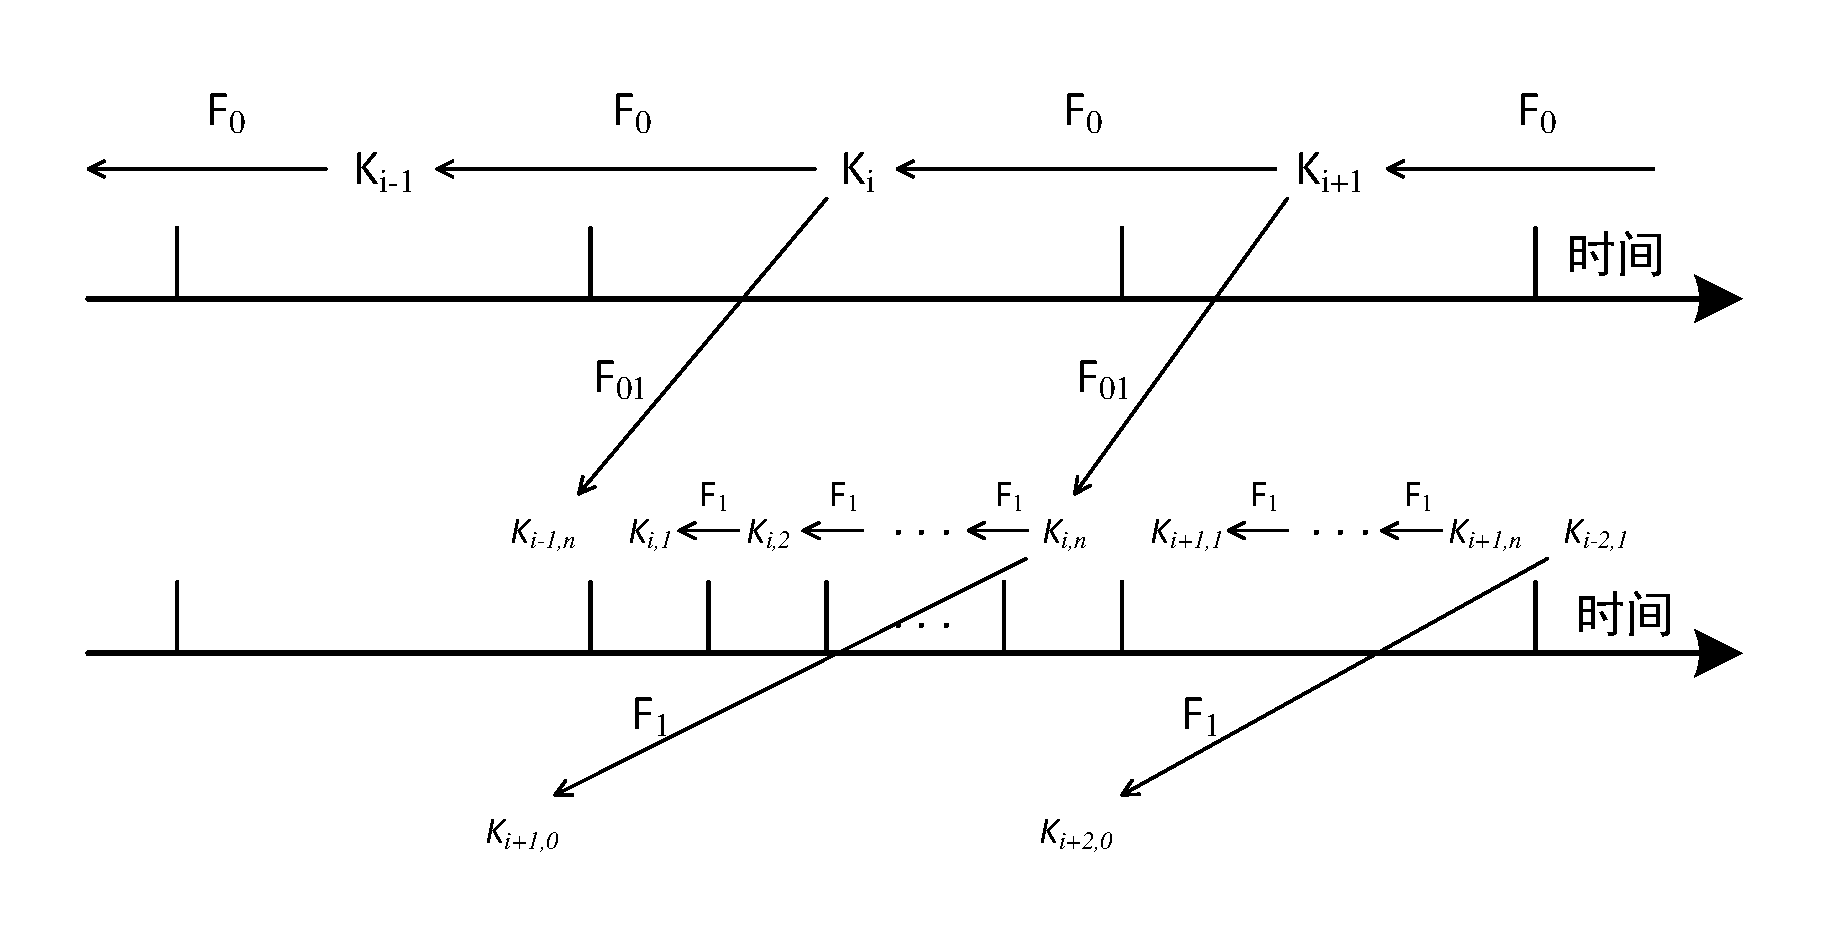
\includegraphics[width=5in]{multiTESLA}
  \caption{多级$\mu TESLA$认证机制}
  \label{fig:MultiTESLA}
\end{figure}

在裴庆祺等人的$\mu TESLA$改进方案中\upcite{c1:MMtesla},引入了$(t,n)$的门限秘密共享,每个认证密钥被分隔为$n$个密钥片,分配到各个基站。在无线传感网中执行原有的$\mu TESLA$方案,将密钥片进行广播,当一个节点接收到超过$t$个密钥片之后,就通过秘密共享的算法,对认证密钥进行恢复,重构出认证密钥。该方案提高了$\mu TESLA$方案的认证率,并且有高可靠性和高容忍性的特点,缺点是通信开销明显增加。

Anas等人提出了一种基于信任模型的认证方案\upcite{c1:anas},使用一个轻量级的基于椭圆曲线的简单认证密钥协议。通过通信实体之间建立信任级别,使非对称密钥认证系统能在资源有限的无线传感器节点上运行。

Dong等人利用消息预认证提出了一个基于密钥链的过滤方案\upcite{c1:verifyfilter},能对无线传感网中的广播进行过滤,有效减少虚假广播对传感网数据传输的影响,该方案的缺点是无法有效防御攻击者的联合节点攻击。




\subsection{无线传感网身份认证概述}

攻击者可以通过对网络发送大量的虚假数据报文,大量消耗节点的计算和存储能力,消耗节点的能量,导致传感网的失效。因此对传感网中的节点进行身份认证尤为重要。
文献\cite{c2:chan2003random}中,利用随机配对密钥分配方案,一个密钥仅会分配给一对节点,来实现一种非常简单的身份认证,即两个节点通过使用预分配的密钥对消息的加密和解密判断是否是经过认证的节点。但是该方案无法实现真正的身份认证,因为被捕获的节点可以伪装成正常节点进行欺骗,对无线传感网进行攻击。

现有的身份认证方案主要有非对称密钥认证和秘密共享认证。
由于无线传感器节点的限制,现阶段非对称密钥认证的实现一般是消耗能量较多的计算由基站完成,消耗能量较少的计算由节点完成。秘密共享的认证则是基于多个节点共同对一个节点进行认证。

虽然现阶段由于传感器节点的限制,非对称密钥没有被广泛应用于无线传感网的认证,但是许多研究也对此进行了探索。
在非对称密钥机制中,椭圆曲线密码(Elliptic Curve Cryptography,ECC)是一种轻量级的方案,研究结果表明,160位的ECC 能获得相当于1024位RSA密码的安全性能。而且使用非对称密钥不需要$\mu TESLA$方案中的延迟发布密钥,还能提高认证系统的安全性。

Watro等人提出了一个基于RSA算法的认证机制TinyPK\upcite{c1:Watro},该方案使用请求-应答机制。
该方案使用了双重校验,来保证认证机制的安全性。
当一个节点需要同另一个节点进行认证时,向该节点发送一个请求信息,其中包括两部分。第一部分是使用认证中心的私钥进行签名的请求节点的公钥,第二部分是使用请求节点私钥签名的时间戳和消息认证码。应答节点接收到该请求消息以后,使用认证中心的公钥对第一部分进行解密,获取请求节点的公钥。使用请求节点的公钥解密第二部分,获得时间戳和消息认证码,通过时间戳和消息认证码的校验,来判断请求节点的合法性。如果通过,则建立两个节点之间的安全通信。

在Bauer等人的方案\upcite{c1:Bauer}中,使用了秘密共享的思想进行身份认证。当一个节点请求对另一个节点的认证时,应答节点发送消息给认证中心,宣告自己被请求做认证处理,处理中心将请求节点的私钥进行划分,将秘密片广播给应答节点的邻居节点,所有节点发回给认证中心一个判定消息,如果通过认证的消息超过阈值,则请求节点通过认证,应答节点此时与认证中心进行交互,更新自己的私钥。

现有的身份认证方案还有Benenson提出的基于ECC的方案\upcite{c1:Benenson},Cao等基于vBNN-IBS提出的多用户广播认证方案\upcite{c1:Cao}。



\section{无线传感网密钥分配方案概述}

\subsection{无线传感网密钥分配概述}
无线传感网的密钥分配是其安全技术研究的一个重要内容,包括密钥预分发、共享密钥发现等研究方向。

无线传感网中的密钥分配与传统无线网络有较大区别,在传统的无线网络中,密钥分配方案的研究已经取得了许多成果,但是由于无法适应无线传感网的特点,这些成果无法应用于无线传感网中。因为WSN节点资源的限制,传统无线网络中节点计算开销和通信开销较大的密钥分配方案无法适用。在设计无线传感网的密钥分配方案时,不仅要保证方案的安全性能,也要权衡计算开销和通信开销。

进行认证的基础是密钥分配,设计一个面向无线传感网需求的密钥分配方案,才能保证认证机制的性能。
\subsection{无线传感网密钥分配方案分类}
近些年来,WSN的密钥分配有了许多新的研究成果,根据所适用的密钥是否是对称密钥,可以将方案分为对称密钥方案和非对称密钥方案。随着传感器技术的发展,非对称密钥技术可能成为将来无线传感器密钥分配的主流,但是由于目前无线传感器节点的计算能力和存储空间的限制,现有的无线传感网密钥分配以对称密钥方案为主。基于对称密钥,有很多的密钥分配机制的研究成果,表~\ref{tb:wsnkey}列出了目前无线传感网主要的密钥分配方案:

\begin{table}[htbp]
  \centering
  \caption{无线传感网主要的密钥分配方案}
  \label{tb:wsnkey}
  \begin{minipage}[t]{0.8\textwidth}
    \begin{tabularx}{\linewidth}{|c|X|X|}
      \hline
%      \multirow{1}*{网络层次}
%        & 常见的攻击 & 防范措施\\
      \multirow{1}*{数学结构}  & \multicolumn{1}{c|}{密钥分配方案} & \multicolumn{1}{c|}{密钥分配方法} \\
      \hline
      \multirow{3}*{密钥池}
        & E-G方案 & 随机预分发 \\\cline{2-2}
        & q-composite方案 & \\\cline{2-3}
        & PIKE方案 & 基于网格预分发\\
      \hline
      \multirow{4}*{二元对称多项式}
        & Blundo方案 & 确定预分发\\\cline{2-3}
        & Liu-Ning方案 & 基于随机子集预分发 \\\cline{2-3}
        & GBKP方案 & 基于网格预分发 \\\cline{2-3}
        & CPKS方案 & 基于位置预分发 \\
      \hline
      \multirow{2}*{MDS 码生成矩阵}
        & Blom方案 & 确定预分发 \\\cline{2-3}
        & Du-Deng方案 & 基于随机子集预分发 \\
      \hline
      \multirow{2}*{区组}
        & Camtepe方案 & 组合设计 \\\cline{2-3}
        & Camtepe混合组合设计方案 & 组合设计及随机预分发 \\
      \hline
    \end{tabularx}\\[2pt]
  \end{minipage}
\end{table}



\subsection{无线传感网典型密钥分配方案概述}
根据密钥分配方法的不同,我们对不同类别的无线传感网密钥分配方案进行概述:
\subsubsection{基于随机预分发的密钥分配}
Eschenauer和Gligor基于随机图理论,提出了无线传感网中随机密钥预分配的方案\upcite{c2:Eschenauer2002}(简称E-G方案),该方案包括3个阶段。在密钥预分发阶段,密钥分发中心生成一个足够大的密钥池$P$,然后对于每个传感器节点,从中随机选择$m$个不同的密钥,形成一个密钥环,并将密钥保存到传感器节点的存储空间中。在密钥发现阶段,每个节点通过相邻节点发现机制寻找物理上相邻的节点,由于所有节点的密钥是从密钥池中随机取出的,相邻节点可能存在相同的密钥,如果相邻节点存在共享密钥,则作为两者之间的会话密钥。当相邻节点之间不存在共享密钥,则开始路径密钥建立阶段。通过在密钥发现阶段建立的节点连通图$G(V,E)$(V为传感器节点的顶点集合,E为有共享密钥的传感器节点之间构成的边集),在图中查找一条通往没有共享密钥的相邻节点的路径,建立相邻节点之间的路径密钥。

在E-G方案中,两个相邻节点之间有共享密钥的概率$p$同节点存储密钥数$m$之间的关系可以表示为:$p=1-\frac{((P-m)!)^2}{(P-2m)!P!}$。E-G 方案使得每个节点只需要存储较小数量的密钥,就可以有较高概率使得无线传感器网络完成密钥建立过程,符合无线传感网的特点要求。但是E-G 方案作为最早提出的无线传感网密钥预分发方案,也有自身的缺点,当妥协节点增多时,无法保证无线传感网的通信安全,因为节点不具备防篡改的机制。而且当一个节点被捕获时,节点上存储的密钥材料全部都暴露给了攻击者,而且这些密钥可能是其他节点间的会话密钥,也就是使攻击者能攻击其他节点之间的通信。

在E-G方案的基础上,有许多方案对随机密钥预分配进行了改进,提升随机密钥预分配机制的性能。
Chan等人在E-G方案的基础上提出了q-composite 随机密钥预分配方案\upcite{c2:chan2003random},每个节点从密钥池$P$中获取$m$个不同的密钥。方案的密钥个数阈值为$q$,当两个节点之间的共享密钥个数$q^{'}$满足$q^{'}> q$,则两个节点之间使用hash函数$K=hash(K_1\| K_2\| \cdots \| K_{q^{'}})$生成会话密钥,在q-composite方案中,hash函数使用了SHA-1\cite{c2:sha1}。q-composite保证了相邻节点之间的安全链路,密钥个数阈值增大时,链路的安全性能也增大。在无线传感网被捕获节点较少时,该方案节点间链路的安全性能比E-G方案更好,但是当被捕获节点增多时,该方案的安全性能明显下降。


在Blom的对称密钥生成方案\upcite{c2:Blom84} 基础上,Du等人将其与随机密钥预分发结合,提出了无线传感网多密钥空间密钥预分发方案\upcite{c2:du2005pairwise}。先使用Blom方案生成$\omega$个密钥空间,每个节点从中选择$\tau$个密钥空间保证在存储空间中$(2 \leq \tau \leq \omega)$,如果两个节点上存储了一个相同的密钥空间,则他们之间计算生成一个共享密钥。与E-G 方案和q-composite方案相比,Du-Deng方案通过计算适合的参数$\omega$和$\tau$,能明显提高抵抗链路攻击的性能,但是同时也增加了节点的计算开销。

Blundo利用二元对称多项式的性质,提出了节点对密钥建立方案\upcite{c2:Blundo1998}。密钥服务器随机生成一个有限域上的$k$ 阶二元对称多项式$f(x,y)=\sum _{i,j=0}^k a_{i,j} x^i y^j$,对于对称多项式,有$f(x,y)=f(y,x)$。对于任意节点$i$,服务器计算$f(i,y)$,然后将$k+1$个系数存入节点存储空间。当节点$i$和节点$j$需要建立对密钥时,计算$f(i,y)$ 在$y=j$ 时的值,计算$f(j,y)$在$y=i$时的值,因为$f(i,j)=f(j,i)$,所以$f(i,j)$就可以作为节点$i$和节点$j$之间的对密钥。

在Blundo方案的基础上,Liu-Ning提出了基于对称二元多项式池的随机密钥预分配方案\upcite{c2:liu2005establishing}。
密钥服务器在有限域$F_q$上随机生成一个二元对称多项式的集合$\phi=\{f_i(x,y),i=1,\cdots,t\}$,对于节点$i$,将子集$\phi_i\subseteq \phi$装入存储空间。当两个节点发现有相同的二元多项式,则直接使用Blundo的节点对密钥建立方案建立会话密钥。当被捕获的节点较少时,Liu-Ning方案有较好的安全性能,但是在攻击者捕获了较多节点,也就是获得较多二元多项式的时候,链路的安全性能相较E-G方案和q-composite方案更低。

利用节点的位置信息,Liu提出了最近对密钥方案(CPKS)\upcite{c2:LiuN03},节点实际分布位置在其期望分布位置周围服从均匀分布。每个节点与自己期望分布位置最近的$t$节点之间建立对密钥,例如,对节点$u$的相邻节点$v$,密钥服务器生成对密钥$K_{u,v}$,并将$u,K_{u,v}$和$v,K_{u,v}$分别存入节点$u$和节点$v$。通过两个节点之间的ID信息可以判断两个节点之间是否存在对密钥。在节点位置信息已知时,该方案相比前述方案有更好的性能,缺点是网络扩展性较差,加入新节点,需要大量节点能量消耗。

Du提出的基于部署知识的方案\upcite{c2:Du06} 中,将密钥池$S$划分为$t\times n$的子密钥池$S_{i,j}(1\leq i\leq t,1\leq j\leq n)$,子密钥空间$S_{i,j}$对应着部署组$G_{i,j}$。根据部署位置的信息,不同的子密钥池之间发现共享密钥。该方案提高了无线传感网中节点链路连通的概率,但是子密钥池的划分对安全性能的影响较大。


\subsubsection{基于网格预分发的密钥分配}
为了解决随机密钥预分配方案中链路密钥的不确定性,Liu提出了基于网格的密钥预分配方案(GBKP)\upcite{c2:LiuND08}。
对一个$m\times n$的传感网,如图~\ref{fig:GBKP}所示,$G_i$为部署分组。对$G_i$中的节点分配ID集合$\{(i-1)m+j|j=1,\cdots,m\}$,对$G_i^{'}$中的节点分配ID集合$\{i+(j-1)m|i=1,\cdots,n\}$。服务器生成$m+n$个对称二元多项式分配给每行每列,使得同一行或同一列的节点能直接生成对密钥,不同行或列的节点,通过中间节点生成链路密钥。
类似的基于网格预分发的密钥分配方案还有Chan 提出的PIKE方案\upcite{c2:ChanP05}。
\begin{figure}[htbp]
  \centering
  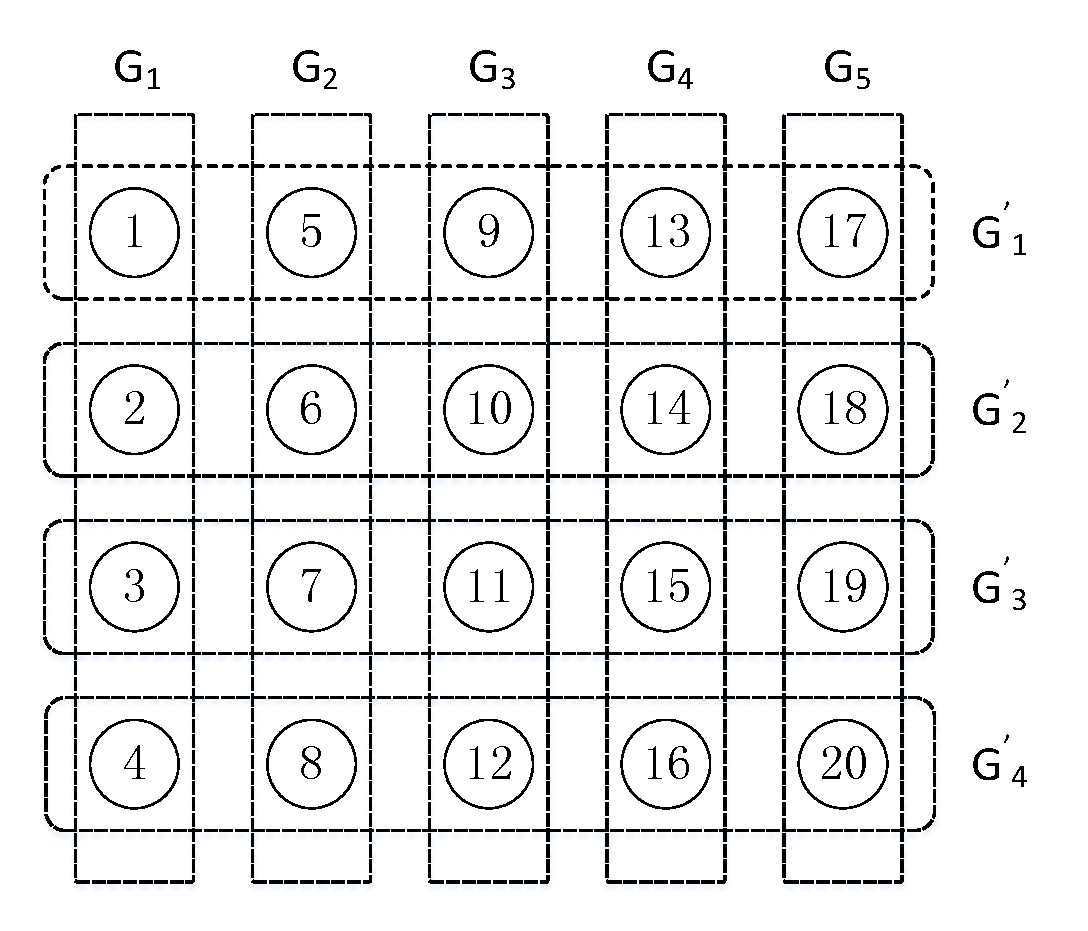
\includegraphics[width=4in]{GBKP}
  \caption{基于网格的密钥预分配方案}
  \label{fig:GBKP}
\end{figure}

\subsubsection{基于组合设计的密钥分配}
Camtepe把组合设计的理论应用于无线传感网的密钥分配\upcite{c2:CamtepeY07},使用组合设计理论来划分密钥池和密钥环。
对一个规模为$N$的无线传感网,生成一个对称BIBD,$(n^2+n+1,n+1,1)$,其中$n$为满足$n^2+n+1\geq N$的最小素数,密钥池的大小为$n^2+n+1$,密钥环的长度为$n+1$。这个方案保证了无线传感网中的任意一对节点有共享密钥,或通过中间节点生成的链路密钥。
为了解决该方案在网络规模方面的限制,Camtepe 还提出了组合设计与广义四边形想结合的方案。


